\documentclass[12pt]{article}
\usepackage{epsfig,verbatim}
\usepackage{color}
\usepackage{algorithm}
\usepackage{algorithmic}
\floatname{algorithm}{Procedure}
%\pagestyle{headings}
\textheight 8.5 in
\topmargin -0.35 in
%\topmargin -0.10 in
\oddsidemargin -0.1 in
\renewcommand{\topfraction}{1}
\renewcommand{\bottomfraction}{1}
\renewcommand{\textfraction}{0}
\renewcommand{\floatpagefraction}{0.90}
\makeatletter
\def\singlespace{\def\baselinestretch{1}\@normalsize}
\def\endsinglespace{}
\newtheorem{lemma}{Lemma}%[section]
\newtheorem{theorem}{Theorem}%[section]
\newtheorem{remark}{Remark}
\newtheorem{example}{Example}%[section]
\newtheorem{corollary}{Corollary}%[section]
\@addtoreset{equation}{section}
\renewcommand{\theequation}{\thesection.\arabic{equation}}
\renewcommand{\thefootnote}{\fnsymbol{footnote}}
\renewcommand{\hat}{\widehat}
\def\singlespace{\def\baselinestretch{1}\@normalsize}
\def\endsinglespace{}
\makeatother
\def\c{\centerline}
\newcommand{\by}{\mbox{\bf y}}
\newcommand{\bX}{\mbox{\bf X}}
\newcommand{\bZ}{\mbox{\bf Z}}
\newcommand{\bz}{\mbox{\bf z}}
\newcommand{\bx}{\mbox{\bf x}}
\newcommand{\bV}{\mbox{\bf V}}
\newcommand{\ba}{\mbox{\bf a}}
\newcommand{\bb}{\mbox{\bf b}}
\newcommand{\pl}{p_{\lambda}}
\newcommand{\bbeta}{\mbox{\boldmath$\beta$}}
\newcommand{\bga}{\mbox{\boldmath$\gamma$}}
\newcommand{\balpha}{\mbox{\boldmath$\alpha$}}
\newcommand{\bpsi}{\mbox{\boldmath$\psi$}}


\newcommand{\btheta}{\mbox{\boldmath$\theta$}}
\newcommand{\hbeta}{\hat{\beta}}
\newcommand{\hbbeta}{\hat{\bbeta}}
\newcommand{\halpha}{\hat{\alpha}}
\newcommand{\htheta}{\hat{\theta}}
\newcommand{\hbtheta}{\hat{\btheta}}
\newcommand{\bW}{\mbox{\bf W}}
\newcommand{\bvar}{\mbox{\boldmath$\varepsilon$}}

% =================== THE SELF-DEFINED COMMANDS =============================
\font\larges=cmbx8 scaled 1500
\def\newpage{\vfill\eject}
 \def\wh{\widehat}
 \def\Var{\mbox{Var}}
\def\MSE{\mbox{MSE}}
 \def\andd{\mbox{and}}
 \def\logit{\mbox{logit}}
\def\new{\mbox{new}}
\def\say{\mbox{(say)}} \def\wt{\widetilde}
\def\today{\ifcase\month\or
  January\or February\or March\or April\or May\or June\or
  July\or August\or September\or October\or November\or December\fi
  \space\number\day, \number\year}
\def\Cov{\mbox{Cov}}  \def\C{\mbox{const.}\quad} \def\no{\noindent}
\def\proof{{\noindent\underbar{\bf Proof}\quad}}
\def\Lemma#1{{\noindent\underbar{\bf Lemma #1}\quad}}
\def\Theorem#1{{\noindent\underbar{\bf Theorem #1}\quad}}
\def\Remark#1{{\noindent\underbar{\bf Remark #1}\quad}}
\def\endp{{\vrule width 5pt height 5pt\par}}
\def\d{\quad{\buildrel  {\cal D}\over\longrightarrow}\quad}
\newdimen\biblioindent    \biblioindent=30pt
\def\bibentry{\hangindent=\biblioindent}
\def\wh{\widehat}
\font\smallfont=cmr8 at 7truept
\def\MLE{\mbox{\smallfont{MLE}}}
\def\U{\mbox{\smallfont{U}}}
\def\sgn{\mbox{sgn}}

\def\bH{{\bf H}}
\def\bU{{\bf U}}
\def\bu{{\bf u}}
\def\bV{{\bf V}}
\def\bI{{\bf I}}
\def\bv{{\bf v}}
\def\bY{{\bf Y}}
\def\diag{\mbox{diag}}
\def\supp{\mbox{supp}}
\def\MSE{\mbox{MSE}}
\def\MMSE{\mbox{MMSE}}
\def\SMSE{\mbox{SMSE}}
\def\cov{\mbox{cov}}
\def\gcv{\mbox{GCV}}
\def\tr{\mbox{tr}}
\def\argmin{\mbox{argmin}}
\def\var{\varepsilon}
\def\la{\lambda}
\def\si{\sigma}
\def\rss{(\bY-\bX\bbeta)^T(\bY-\bX\bbeta)}
\newcommand{\be}{\begin{equation}}
\newcommand{\ee}{\end{equation}}
\newcommand{\beq}{\begin{equation}}
\newcommand{\eeq}{\end{equation}}
\newcommand{\beqn}{\begin{eqnarray}}
\newcommand{\eeqn}{\end{eqnarray}}
\newcommand{\beqnn}{\begin{eqnarray*}}
\newcommand{\eeqnn}{\end{eqnarray*}}

\newtheorem{thm}{Theorem}[section]
\newtheorem{lem}{Lemma}[section]
\newtheorem{rem}{Remark}[section]
\newtheorem{cor}{Corollary}[section]
\newtheorem{exam}{Example}[section]
\newtheorem{ass}{Assumption}[section]
\newtheorem{prop}{Proposition}[section]

\def\S{{\bf A}}
\def\s{{\bf a}}
\def\eps{\varepsilon}

\newcommand{\pln}{p_{\lambda_n}}
\newcommand{\etal}{{\it et al }}
\newcommand{\eg}{{\it e.g. }}
\newcommand{\what}{\widehat}

% ================END OF THE SELF-DEFINED COMMANDS =====================

% ================END OF THE SELF-DEFINED COMMANDS =====================

\begin{document}
\renewcommand{\baselinestretch}{1.5}

\title{MDA project}
\author{John Ensley, Mohammad Mottahedi and Songshan Yang}

\date{\today}
\maketitle
\section{Introduction of the data set}

In this project, we applied the mixture discriminant analysis (MDA), linear discriminant analysis and quadratic discriminant analysis (QDA) for to the breast cancer data set. This breast cancer databases was obtained from the University of Wisconsin Hospitals, Madison from Dr. William H. Wolberg.
There are $699$ subjects in the data set and all the subjects are classified to $2$ different classes--"Benign" and "Malignant". There are $9$ features include clump thickness, uniformity of cell size, uniformity of cell shape, marginal adhesion, single epithelial cell Size, bare nuclei, bland chromatin, normal nucleoli, mitoses and all of them range from $1$ to $10$.

\section{Pseudocode}
The pseudocode of the EM algorithm of MDA is shown below:
\begin{algorithm}
	\caption{EM algorithm for MDA}
	\label{alg:1}
	\begin{algorithmic}
		\REQUIRE $X =$ matrix of covariates; $Y =$ class; $R =$ number of subclasses in each class
		\ENSURE $\pi =$ mixture weights; $\mu =$ subclass means; $\Sigma =$ shared subclass variance
		\STATE $K :=$ number of classes
		\STATE $m :=$ number of covariates
		\STATE $n :=$ number of observations
		\STATE $\Sigma = I_{m \times m}$
		\FOR{$k=1$ \TO $K$}
		\STATE $X^* =$ rows of $X$ that belong to class $k$
		\STATE $\mu_{k1},\dots,\mu_{kr} =$ result from $k$-mean clustering on $X^*$ with $R$ clusters
		\STATE $\pi_{k1},\dots,\pi_{kr} = 1/R$
		\ENDFOR
		\WHILE{likelihood has not converged}
		\FOR{$i=1$ \TO $n$}
		\STATE $k :=$ class that $x_i$ belongs to
		\FOR{$r=1$ \TO $R$}
		\STATE $p_{i,r} = \frac{\pi_{kr} \phi(x_i|\mu_{kr},\Sigma)}{\sum_{r'=1}^R \pi_{kr'} \phi(x_i|\mu_{kr'},\Sigma)}$
		\ENDFOR
		\ENDFOR
		\FOR{$k=1$ \TO $K$}
		\STATE $X^* =$ rows of $X$ that belong to class $k$
		\FOR{$r=1$ \TO $R$}
		\STATE $\pi_{kr} = \frac{\sum_{i=1}^n I(X_i \in X^*)p_{ir}}{\sum_{i=1}^n I(X_i \in X^*)}$
		\STATE $\mu_{kr} = \frac{\sum_{i=1}^n X_i I(X_i \in X^*)p_{ir}}{\sum_{i=1}^n I(X_i \in X^*) p_{ir}}$
		\STATE $\Sigma = \frac{\sum_{i=1}^n \sum_{r=1}^R p_{ir}(X_i - \mu_{kr})(X_i - \mu_{kr})'}{n}$
		\ENDFOR
		\ENDFOR
		\ENDWHILE
		\RETURN $\pi$, $\mu$, $\Sigma$
	\end{algorithmic}
\end{algorithm}

\begin{algorithm}
	\caption{MDA}
	\label{alg:2}
	\begin{algorithmic}
		\REQUIRE $\pi =$ mixture weights; $\mu =$ subclass means; $\Sigma =$ shared subclass variance; $X =$ new covariate matrix
		\ENSURE $Y =$ classification labels for $X$
		\STATE $K :=$ number of classes
		\STATE $n :=$ number of observations
		\STATE $R :=$ number of subclasses in each class
		\FOR{$i=1$ \TO $n$}
		\FOR{$k=1$ \TO $K$}
		\STATE $p_k = \sum_{r=1}^R \pi_{kr} \phi(X_i|\mu_{kr},\Sigma)$
		\ENDFOR
		\STATE $Y_i = \arg\max_k p_k$
		\ENDFOR
		\RETURN $Y$
	\end{algorithmic}
\end{algorithm}
We use R programming to finish the algorithm by following the above pseudocode.

\newpage
\section{Mixture Discriminant Analysis}
In the first step, we applied MDA to the whole data set to examine their classification error rate. We found that there are only $16$ subjects having missing data and we delete these subjects, since the results will not be affected because of the large sample size.

There are $458$ subjects belonging to Benign and $241$ subjects belonging to Malignant, so the prior probabilities are $\pi_1=0.65$ and $\pi_2=0.35$ for benign and malignant, respectively.

We changed the number of components in each mixture distribution from $1-6$. the models were trained on 60 percent of the data and the rest of the data was used for testing the accuracy. Figure \cite{mda_acc} show the mixture discriminant accuracy with respect to number of components.

\begin{figure}
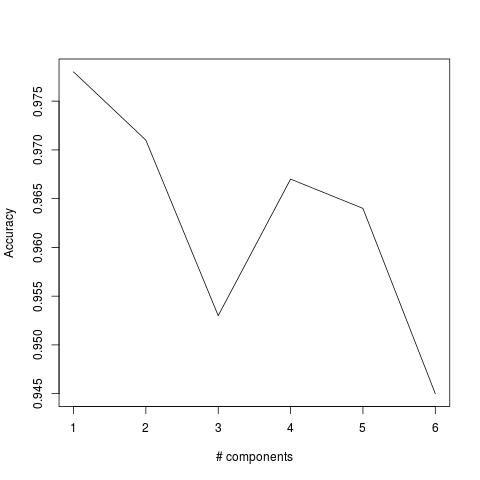
\includegraphics[scale=.8]{mda_acc.jpeg}
\caption{Mixture discriminant analysis accuracy}
\label{mda_acc}
\end{figure}

The model with single component mixture distribution has the best accuracy on the test set. Increasing the number of component does not improve the accuracy.

Next, we used principle component analysis to reduce the dimentionality and used the first two component which allows us to visually inspect the the model. The first two component of the principal component analysis can describe $76.2\%$ of the variation in the data. Figure \cite{pca} shows the result applying principal component analysis on the data set.
\begin{center}
\begin{figure}
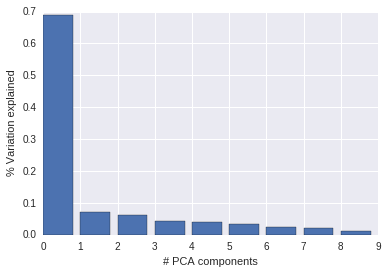
\includegraphics[scale=.8]{pca.png}
\caption{Principal Component analysis}
\label{pca}
\end{figure}
\end{center}
The accuracy of MDA applied to the first two component of PCA is shown in Figure \cite{pca_acc}

\begin{figure}
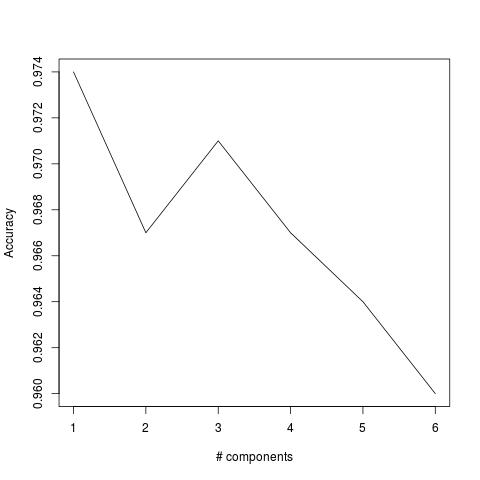
\includegraphics[scale=.8]{pca_acc.jpeg}
\caption{Mixture discriminant analysis accuracy after PCA}
\label{pca_acc}
\end{figure}

Dimensional reduction did not improved the accuracy.

\section{Quadratic , Linear Discriminant Analysis, Logistic Regression, CAR}

To compare the performance of the Mixture discriminant analysis we also trained Quadratic and Linear discriminant analysis on the breast cancer data set.  For LDA, we compute the means of the class "Benign" and "Malignant" and the covariance matrix of the $9$ features. Then we classify the subjects according to the maximum of their discriminant functions. For QDA, the process is similar to that of LDA, but we should compute the covariance matrix for each class and then classify the subjects.

The classification results are summarized in Table \ref{tab1}.

\begin{table}[htbp]
\begin{center}
\caption{\label{tab1} Classification Error Rate of LDA, QDA and Logistic Regression}
\begin{tabular}{c|ccccc}
				\hline
Method&MDA&CART&LDA &QDA &Logistic Regression \\
				\hline
Error Rate& 0.978  &0.949&0.9605&0.974&0.9693  \\
				\hline
\end{tabular}
\end{center}
\end{table}


From Table \ref{tab1}, we can see that MDA and QDA have similar classification error rates and MDA and QDA outperforms the logistic regression and LDA and CART in the classification, CART performs the worst.


\section{PCA on LDA, QDA and Logistic regression}
In this section, we examined the effect of dimension reduction on classification. We first standardized the design matrix and did eigen decomposition of the covariance matrix of the standardized design matrix.

We decided to use the first two components which account for $76.2$\% of the total variance. Then the design matrix only has two columns. By repeating the process described in section 2, the classification error rates are summarized in Table \ref{tab3}. All the simulation results are based on 100 independent replicates.
\begin{table}[htbp]
	\begin{center}
		\caption{\label{tab3} Classification Error Rate of LDA, QDA and Logistic Regression}
		\begin{tabular}{c|ccccc}
			\hline
			Method&MDA &CART&LDA &QDA &Logistic Regression \\
			\hline
			Error Rate&0.974&0.9498&.9605&0.9677&0.9693  \\
			\hline
		\end{tabular}
	\end{center}
\end{table}
Compared Table \ref{tab3} and Table \ref{tab1}, we can see that PCA decreased the accuracy of the QDA slightly, and it does not have effect on MDA, LDA and Logistic regression.

\section{Conclusion}
From the results, we can see that MDA outperforms LDA and QDA in the classification and PCA method did not improve the performance of MDA.



\end{document}
